\begin{pastexam}[label={px:ntust-109-et-ds-02}]{臺科大電子所甲組 109 學年度 第 2 題}
（問答；20 分）

Heaps are a kind of data structure. Answer each of the following questions:
\begin{enumerate}[label=(\alph*)]
\item Define a heap. (6\%)
\item Using the following data, construct a heap: (7\%)

\quad 43\quad 21\quad 5\quad 7\quad 24\quad 31\quad 6\quad 9\quad 32\quad 12
\item Store the above heap in a one-dimensional array. (7\%)
\end{enumerate}
\end{pastexam}

\begin{pastsoln}
題目沒有指定最大或最小堆積，也沒有指定建法。 本書以\textbf{最大堆積、依序插入}作答，最後附上
其他做法的結果。 作答時第一行寫明採用哪一種。

\textbf{(a) 定義。} 堆積是一棵\textbf{完整二元樹}（除了最後一層都填滿，最後一層的節點靠左），
而且滿足\textbf{堆積性質}：最大堆積中每個節點的鍵都不小於它的子節點（最小堆積則不大於）
（資結書定義~8.1、第~8.1~節）。 因此最大堆積的根是最大值。 完整二元樹可以不用指標，直接
依層序存在陣列 $A[1..n]$：$A[i]$ 的父節點在 $A[\lfloor i/2 \rfloor]$，子節點在 $A[2i]$、
$A[2i + 1]$。

\textbf{(b) 建立最大堆積（依序插入）。} 每次把新的鍵放在最後一格，若比父節點大就和父節點交換，
一直往上（資結書第~8.1~節的插入）。 下表的陣列是每次插入完成後的 $A[1..]$：
\begin{center}
\small
\begin{tabular}{cll}
\toprule
插入 & 往上換的過程 & 之後的陣列 \\
\midrule
43 & 第一個 & 43 \\
21 & $21 < 43$，不換 & 43, 21 \\
5 & $5 < 43$ & 43, 21, 5 \\
7 & 放在 $A[4]$，父 $A[2] = 21$，不換 & 43, 21, 5, 7 \\
24 & $A[5]$，父 $21$：換；父 $43$：不換 & 43, 24, 5, 7, 21 \\
31 & $A[6]$，父 $5$：換；父 $43$：不換 & 43, 24, 31, 7, 21, 5 \\
6 & $A[7]$，父 $31$：不換 & 43, 24, 31, 7, 21, 5, 6 \\
9 & $A[8]$，父 $7$：換；父 $24$：不換 & 43, 24, 31, 9, 21, 5, 6, 7 \\
32 & $A[9]$，父 $9$：換；父 $24$：換；父 $43$：不換 & 43, 32, 31, 24, 21, 5, 6, 7, 9 \\
12 & $A[10]$，父 $21$：不換 & 43, 32, 31, 24, 21, 5, 6, 7, 9, 12 \\
\bottomrule
\end{tabular}
\end{center}
最後的最大堆積：
\begin{center}
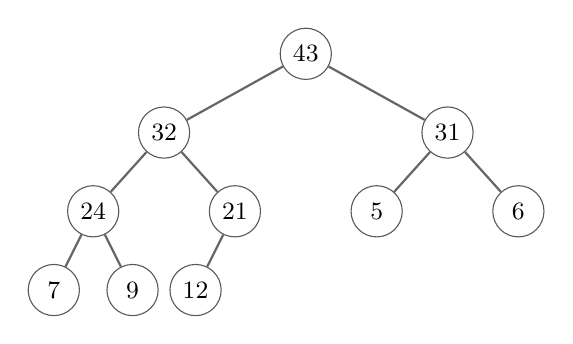
\begin{tikzpicture}[
    hn/.style={circle, draw=black!65, line width=0.4pt, minimum size=6.5mm, inner sep=0pt, font=\small},
    level distance=10mm, edge from parent/.style={draw=black!60, thick},
    level 1/.style={sibling distance=36mm}, level 2/.style={sibling distance=18mm},
    level 3/.style={sibling distance=10mm}]
\node[hn] {43}
    child {node[hn] {32}
        child {node[hn] {24} child {node[hn] {7}} child {node[hn] {9}}}
        child {node[hn] {21} child {node[hn] {12}} child[missing] {}}}
    child {node[hn] {31}
        child {node[hn] {5}}
        child {node[hn] {6}}};
\end{tikzpicture}
\end{center}
檢查：每個節點都不小於子節點（$43 \ge 32, 31$；$32 \ge 24, 21$；$31 \ge 5, 6$；$24 \ge 7, 9$；
$21 \ge 12$），形狀是 $10$ 個節點的完整二元樹。

\textbf{(c) 存成一維陣列。} 依層序由左到右：
\begin{center}
\begin{tabular}{c|cccccccccc}
$i$ & 1 & 2 & 3 & 4 & 5 & 6 & 7 & 8 & 9 & 10 \\
\hline
$A[i]$ & 43 & 32 & 31 & 24 & 21 & 5 & 6 & 7 & 9 & 12 \\
\end{tabular}
\end{center}
例如 $A[4] = 24$ 的子節點是 $A[8] = 7$、$A[9] = 9$，父節點是 $A[2] = 32$。 用 C 的 $0$ 起算陣列
時整體往前一格，子節點是 $2i + 1$、$2i + 2$。

\textbf{其他做法的結果。} 由下而上建堆積（資結書第~8.2~節，$O(n)$）：先把資料原樣放進陣列，
從 $i = \lfloor 10/2 \rfloor = 5$ 往回到 $1$ 逐一往下調整。 $i = 5$（24，子 12）不動；$i = 4$
（7，子 9、32）和 32 換；$i = 3$（5，子 31、6）和 31 換；$i = 2$（21，子 32、24）和 32 換，換下去
後子節點是 9、7，不再換；$i = 1$（43）不動。 得到
\[
43, 32, 31, 21, 24, 5, 6, 9, 7, 12,
\]
也是合法的最大堆積，但和依序插入的結果不同（第 4、5、8、9 格）。 兩種建法的結果本來就可能
不一樣，都算對。 若要最小堆積，依序插入得 $5, 7, 6, 9, 12, 31, 21, 43, 32, 24$；由下而上建得
$5, 7, 6, 9, 12, 31, 43, 21, 32, 24$。
\end{pastsoln}
